\documentclass[conference]{IEEEtran}
\usepackage{amsmath,amssymb,amsthm,booktabs,graphicx,url}
\usepackage{xcolor}
\definecolor{Navy}{HTML}{17324D}
\definecolor{Teal}{HTML}{087F8C}
\definecolor{Coral}{HTML}{B74735}
\definecolor{PaleBlue}{HTML}{EDF5F8}
\renewcommand{\arraystretch}{1.12}
\newcommand{\takeaway}[1]{\begin{center}\setlength{\fboxsep}{9pt}\colorbox{PaleBlue}{\parbox{0.94\textwidth}{\color{Navy}#1}}\end{center}}


\pagestyle{plain}
\emergencystretch=2em
\newtheorem{theorem}{Theorem}
\title{\color{Navy}Formal Verification of Economic Invariants in Decentralized Finance:\\Proving Resilience Against Single-Block Flash-Loan Exploits}
\author{\IEEEauthorblockN{Student research project}\IEEEauthorblockA{Formal methods and blockchain cybersecurity\\\textcolor{Teal}{Visual edition -- September 2026}}}
\begin{document}
\maketitle
\begin{abstract}
Economic verification requires more than preservation of an automated market
maker's reserve invariant. An adversary may restore reserves after a transient
oracle distortion while leaving an undercollateralized debt position elsewhere.
We present an exact-arithmetic prototype for a bounded, single-transaction
constant-product market maker and lending composition. Explicit collateral
forfeiture and flash repayment accounting yield a piecewise convex profit
function. We prove a finite candidate characterization of profitable executions,
a sufficient reserve-depth bound, and conditional security results for bounded
oracles and rational dynamic loan-to-value ratios. A Python/Z3 implementation
checks the existential negation of economic safety and independently replays
rational counterexamples. A synthetic sweep evaluates 90 configurations with
three repetitions each. Separate vault-valuation and donation-health abstractions
illustrate different invariant failures. The artifact is a model-level study:
it does not reproduce historical contract executions, establish bytecode
refinement, or prove that deployed TWAP implementations satisfy its assumptions.
\end{abstract}
\begin{IEEEkeywords}
DeFi security, flash loans, economic invariants, formal verification, Z3.
\end{IEEEkeywords}

\section{\textcolor{Navy}{Introduction}}
Flash loans make substantial temporary liquidity available within an atomic
transaction. Prior work analyzed this capability and the February 2020 bZx
incidents~\cite{qin}. Atomicity guarantees reversal on transaction failure;
it does not imply economic safety for a transaction that successfully repays
its flash lender. A lending protocol can accept a manipulated price while
every executed operation conforms to its local interface.

Economic and programming vulnerabilities overlap. Harvest's incident account
describes share acquisition under manipulated valuation~\cite{harvest}.
Euler's account identifies a missing donation health check~\cite{euler}.
Accordingly, we do not characterize every flash-loan incident as independent
of coding errors. Nor do we infer risk-free realized profit from an oracle
distortion alone: repayment, collateral acquisition, fees, and debt settlement
must be represented.

This study contributes an inspectable accounting model, a closed-form candidate
reduction for its capped profit function, conditional mitigation theorems, and
an executable artifact linking analytical results to solver decisions. These
are modest model-level contributions. Mechanized economic analysis already
exists~\cite{clockwork,defiposer}; applying SMT to DeFi is not itself a novelty
claim. The present draft is a reproducible starting point for stronger
contract-level research, not evidence of venue-level novelty or completeness.

\subsection{\textcolor{Teal}{Research questions}}
The study asks three concrete questions. First, can a reserve-preserving atomic
round trip still yield positive extraction from an attached lender? Second,
which oracle and collateral policies exclude that extraction in the model?
Third, do executable solver decisions agree with the analytical criterion over
a controlled parameter grid? These questions concern integrity of collateral
valuation and preservation of lender assets, placing the work within blockchain
cybersecurity and adversarial economic verification.

\section{\textcolor{Navy}{Threat Model and System Assumptions}}
The adversary chooses a flash amount $0<f\leq F$ and a feasible borrowing amount
in one fixed transaction schedule. It owns $C$ units of collateral token $A$
before execution. Token $B$ is the numeraire.\footnote{All monetary quantities are normalized token units. They are not measured dollar losses or historical exploit proceeds.} The attacker may pledge $C$,
borrow $B$, restore AMM reserves, repay its flash loan, and abandon pledged
collateral under non-recourse ordinary debt. An external reference price
$p_0=y/x$ remains fixed. The opportunity cost of collateral is $V=Cp_0$.
This explicitly states how an outstanding debt becomes extraction: all
collateral is forfeited and there is no additional recourse against the wallet.

The adversary controls operation parameters but cannot forge balances or
violate transition guards. This resembles the adversarial scheduling perspective
of symbolic protocol analysis; we do not give a Dolev--Yao cryptographic term
algebra. The fixed core schedule is not an enumeration of all possible call
sequences. External arbitrage, token transfers with fees, rebases, gas,
concurrent transactions, oracle governance, and cross-block strategies are
excluded. The AMM has no swap fee; the flash fee is $r\geq0$. Borrowing liquidity
is bounded by $T$. Atomic rollback rejects executions unable to repay the
flash obligation, while ordinary debt may persist.

If ordinary debt must also be repaid, the attack analyzed here disappears:
the borrow transfer cancels its repayment and the reserve-restoring round trip
loses only the flash fee. This alternative settlement rule is outside our
default extraction objective and demonstrates why the threat model matters.

\section{\textcolor{Navy}{Theoretical Framework and Constraint Encoding}}
\begin{table}[t]
\centering\caption{Notation and baseline configuration.}
\begin{tabular}{lll}\toprule
\textcolor{Navy}{Symbol} & \textcolor{Navy}{Meaning} & \textcolor{Navy}{Baseline}\\\midrule
$x,y$ & AMM token reserves & 1000, 1000\\
$C$ & Pre-owned collateral & 100\\
$p_0$ & Reference price $y/x$ & 1\\
$V$ & Initial collateral value & 100\\
$L$ & Loan-to-value limit & 0.75\\
$r$ & Flash fee rate & 0.0009\\
$F$ & Flash capacity & 1000\\
$T$ & Lending cash & 400\\
$f,b$ & Chosen flash loan, borrowing & Variables\\
$\Pi$ & Extraction net of initial wealth & $b-rf-V$\\
\bottomrule\end{tabular}\end{table}
\subsection{\textcolor{Teal}{State transitions and accounting}}
State comprises AMM reserves, liquid attacker wallets, lending cash, collateral
custody, ordinary debt, and the flash obligation. Initially the attacker holds
$(C,0)$ and reserves are $(x,y)$, with $x,y>0$. Inputting $A$ decreases $y/x$;
to inflate the price of collateral $A$, the flash loan must instead supply $B$:
\begin{align}
y_1&=y+f,&x_1&=\frac{xy}{y+f},\\
a&=\frac{xf}{y+f},&p_1&=p_0(1+f/y)^2.
\end{align}
After acquisition and swap the wallet is $(C+a,0)$. Pledging $C$ and borrowing
$b$ leaves $(a,b)$, subject to
\begin{equation}0\leq b\leq T,\qquad b\leq C L p_1,\qquad 0<L<1.\end{equation}
Selling all $a$ back restores both reserves and returns exactly $f$, since
$(y+f)a/(x_1+a)=f$. The wallet becomes $(0,b+f)$ before flash repayment and
$(0,b-rf)$ afterwards. The flash lender gains $rf$; the lending protocol has
cash $T-b$, collateral $C$, and a claim for debt $b$. After collateral
forfeiture the attacker's extraction net of initial wealth is
\begin{equation}\Pi=b-rf-V.\end{equation}
This accounting neither charges the recovered principal twice nor treats
pre-owned collateral as free. Feasibility requires $b-rf\geq0$.

\subsection{\textcolor{Teal}{Safety and optimality}}
Let $A_0=VL$. For $C>0$, maximal feasible extraction at each $f$ is
\begin{equation}g(f)=\min\{T,A_0(1+f/y)^2\}-V-rf.\end{equation}
To verify $\forall f,\ \mathrm{Feasible}(f)\Rightarrow\Pi(f)\leq0$, the
solver checks the existential negation with $\Pi>0$. Any positive value of
$g$ automatically satisfies flash repayment. On the uncapped branch,
\begin{align}
g'(f)&=2A_0/y+2A_0 f/y^2-r,\\
g''(f)&=2A_0/y^2>0.
\end{align}
SymPy derives $f_{\mathrm{stationary}}=ry^2/(2A_0)-y$. This point, if in
the branch, is a minimum. Solving a derivative equation alone would therefore
give the wrong attack optimization procedure.

\begin{theorem}[Candidate reduction]
The supremum of $g$ on $(0,F]$ is attained among the endpoint limit $g(0)$,
$g(F)$, and $g(f_c)$ when $f_c=y(\sqrt{T/A_0}-1)$ lies in $[0,F]$.
If $T<A_0$, endpoints alone suffice. A profitable execution exists exactly
when the largest candidate value is positive.
\end{theorem}
\begin{proof}
Before the cash cap binds, strict convexity places the maximum of any closed
subinterval at an endpoint. After the cap binds, the slope is $-r\leq0$.
Split $[0,F]$ at the binding point when present. For $T<A_0$ the entire
interval is capped. Finally, $g(0)\leq V(L-1)<0$, so a positive supremum
must occur at a nonzero allowed candidate. The case $C=0$ separately gives
$b=0$ and no positive extraction.
\end{proof}

For $x=y=1000,C=100,L=3/4,r=9/10000,F=1000,T=400$, the optimal candidate
is $f=1000$. It gives $a=500,p_1=4,b=300$ and profit $1991/10$ units of $B$.
These normalized numbers are constructed, not historical exploit parameters.
The strict positivity test treats equality as safe for this particular objective.

\subsection{\textcolor{Teal}{Conditional mitigation proofs}}
\begin{theorem}[Bounded oracle]
If $0<p_{\mathrm{oracle}}\leq p_0(1+\epsilon)$ and $L(1+\epsilon)\leq1$,
then every allowed execution satisfies $\Pi\leq0$.
\end{theorem}
\begin{proof}
$b\leq CLp_0(1+\epsilon)\leq V$ implies $\Pi\leq-rf\leq0$.
\end{proof}
The property is an oracle assumption. It is not derived from a concrete TWAP
observation implementation. A bound with excessive $\epsilon$ can remain
exploitable and is included as a negative control.

An alternative policy $L(f)=L_0/(1+f/y)^2$ cancels the modeled distortion,
giving $b\leq VL_0<V$. For the proposed exponential policy,
$L(f)=L_0e^{-\lambda f}$, the inequality $\log(1+u)\leq u$ gives the sufficient
condition $\lambda\geq2/y$. This is a separate analytic theorem.\footnote{A conditional proof assumes its oracle or policy bound. A deployment must establish that assumption independently.} Exponentials
are not polynomials and are not encoded exactly in QF\_NRA~\cite{z3}.

\subsection{\textcolor{Teal}{Liquidity bound}}
Fix $p_0,V,L,r,F$. Removing the cash cap upper-bounds profit. Requiring the
uncapped value at $F$ to be nonpositive yields
\begin{equation}
y_{\mathrm{safe}}=\frac{F}{\sqrt{(V+rF)/(VL)}-1},\qquad
k_{\mathrm{safe}}=\frac{y_{\mathrm{safe}}^2}{p_0}.
\end{equation}
The denominator is positive. Convexity and the negative zero endpoint prove
safety for all $f\leq F$ whenever $y\geq y_{\mathrm{safe}}$. The bound is
necessary and sufficient for the uncapped objective, but merely sufficient
when $T$ binds. If $T\leq V$, extraction is already impossible at any depth.
TVL alone specifies neither collateral value nor flash capacity; $k$ alone
does not specify reserve depth without a price normalization. Thus no general
$k_{\min}(\mathrm{TVL})$ follows. With unbounded flash size, zero flash fees,
and $T>V$, every finite pool eventually admits profitable cap-reaching distortion.

\subsection{\textcolor{Teal}{Composable conservation}}
Conservation applies to each underlying token over all wallets and custodians.
An internal transfer debits one balance and credits another; induction over a
finite transition sequence preserves their sum. Gross outflow is not conserved,
because assets may traverse several pools. Debt claims are not new underlying
tokens. Fixed reference prices permit weighting token conservation, while
manipulated spot prices cannot define the conserved valuation.

The auxiliary DAG encoder processes a topological list of swaps with shared
wallets, supporting branches and merges without double spending. Each pool is
used once in this module. Its terminal wallets are separate from the core
lending objective; composing arbitrary borrowing and liquidation actions is
not implemented. The fixed core trace handles its own pool reversal.

\section{\textcolor{Navy}{Prototype Implementation and Z3 Engine}}
The Python artifact separates AMM primitives, borrowing limits, the verifier,
analytical results, integer arithmetic, and experiment drivers. Real arithmetic
uses exact rational constants parsed from decimal text. Positive-denominator
relations are cross-multiplied, for example
$(y+f)(x-a)=xy$. No division by an unconstrained denominator is permitted.
Reserve bounds narrow the search domain; they do not linearize polynomial
products. The engine uses \texttt{SolverFor("QF\_NRA")} with a 30-second
timeout per check. It records SAT, UNSAT, or UNKNOWN without coercing UNKNOWN
to safety, and exports SMT-LIB queries and Z3 statistics.

SAT models are counterexamples, not optimizers. The separate SymPy candidate
procedure supplies optimality for the core model. Rational SAT models are
replayed using Python Fraction arithmetic, checking loan limits, output,
oracle price, borrowing, reversal, and terminal profit. Algebraic irrational
witnesses are not silently rounded: the replay routine rejects unsupported
Fraction input. The measured sweep produced replayable rational witnesses.
UNSAT trusts Z3 and the encoding; this artifact does not emit independently
checked proof certificates or prove source-to-model equivalence.

The optional QF\_BV module checks concrete unsigned 256-bit round-trip traces
using UDiv and widened overflow guards for the specified expression order.
Overflow causes trace rejection under checked arithmetic. For
$q=\lfloor xf/(y+f)\rfloor$, the returned quantity
$\lfloor(y+f)q/x\rfloor\leq f$, proving that this isolated rounding pattern
cannot create round-trip gain. This does not establish rounding safety for
lending, vaults, or other Solidity expressions. The concentrated-liquidity
primitive is restricted to one active range with positive square-root prices;
it is not a full Uniswap v3 implementation~\cite{uniswap}.

\section{\textcolor{Navy}{Case Studies and Evaluation}}
\subsection{\textcolor{Teal}{Historical motivation and abstraction fidelity}}
The bZx-inspired benchmark represents transient spot-price inflation before
borrowing. Prior flash-loan research analyzes the actual incidents~\cite{qin};
our parameters are synthetic. No original contract addresses, archive states,
or transaction replays are used, so model witnesses cannot be described as
historical exploit payloads.

Harvest's account describes favorable share acquisition followed by exit at
regular valuation~\cite{harvest}. Our proxy manipulates two independent CPMMs
and defines $q$ as their average normalized post-swap price. With true initial
assets $A=1000$, supply $S=1000$, and deposit $d=100$, minted shares satisfy
$s(qA)=dS$. At restored valuation redemption satisfies
$R(S+s)=s(A+d)$. Both total assets and supply include the new deposit.
Manipulation loans reverse exactly; profit subtracts repayment of the deposit
loan and all flash fees. The fixed variant mints using $A$ instead of $qA$,
so $R=d$ and positive fee-net profit is impossible. The proxy does not implement
Curve StableSwap, Harvest strategy accounting, or actual manipulation costs.

Euler's own report identifies the missing donation health check~\cite{euler}.
Our example starts with collateral 100 and debt 70 under health factor
threshold $L=0.8$. A positive donation decreases collateral without reducing
debt, allowing $70>0.8C_{\mathrm{after}}$. Adding the post-donation health guard
makes this counterexample impossible. This checks reachability of an unhealthy
state, not profitable self-liquidation. Complete leverage, reserve claims,
discounts, debt migration, and liquidation settlement are absent. Its SAT
decision must not be combined with the core profit results as though both
proved the same property.

\subsection{\textcolor{Teal}{Experimental design and measured results}}
We sweep equal reserves $x=y\in\{100,1000,10000\}$, LTV from 0.50 through
0.95 by 0.05, and flash fees $0.0009,0.0015,0.003$. Collateral is 100,
flash capacity 1000, and lending cash 400. Each of the 90 configurations is
checked three times sequentially. Every decisive result is compared with the
analytical criterion, and every core SAT witness undergoes exact replay.
The sweep returned 204 SAT, 66 UNSAT, and 0 UNKNOWN decisions across 270 checks. All SAT witnesses replayed exactly and all decisions agreed with the analytic criterion.
\begin{table}[t]\centering\caption{Measured core results; 90 checks per reserve scale.}\begin{tabular}{rrrrr}\toprule
\textcolor{Navy}{$x=y$} & \textcolor{Navy}{SAT} & \textcolor{Navy}{UNSAT} & \textcolor{Navy}{Med. ms} & \textcolor{Navy}{Max ms}\\\midrule
100 & 90 & 0 & 20.606 & 52.619\\
1000 & 90 & 0 & 20.785 & 43.826\\
10000 & 24 & 66 & 2.233 & 29.053\\
\bottomrule\end{tabular}\end{table}

\begin{figure*}[t]
\centering
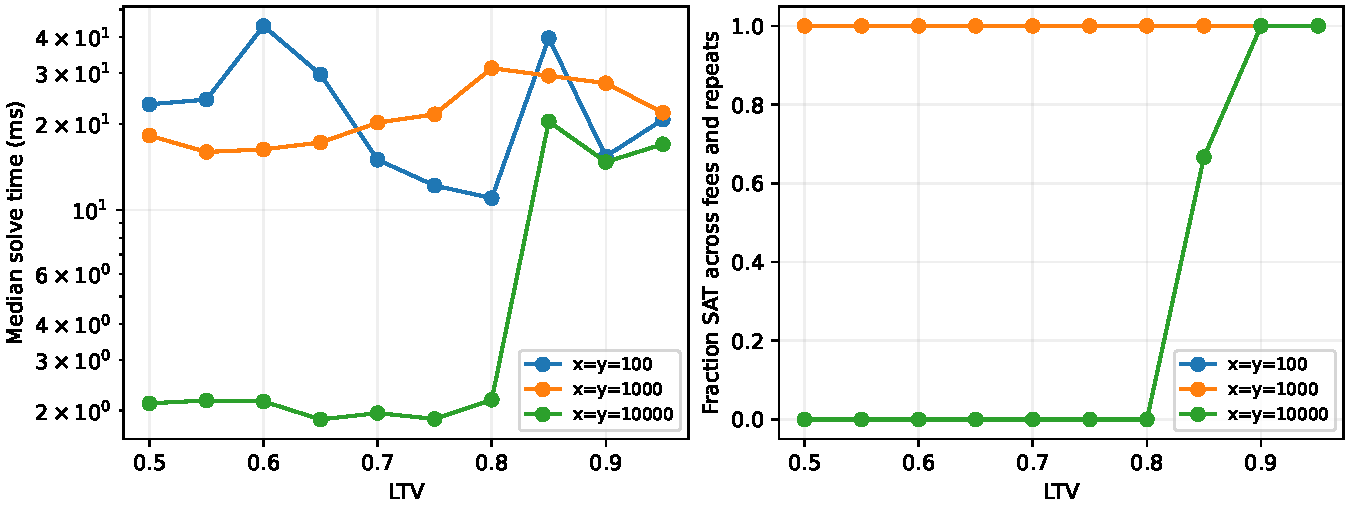
\includegraphics[width=\textwidth]{figures/sweep.pdf}
\caption{Measured median solving time and SAT fraction by LTV. Fractions pool
the three fee values and three repetitions; they are not attack probabilities.}
\end{figure*}

The extended visual analysis provides a decision map, timing distributions, and an explicit wealth ledger.

The test suite additionally checks tight and loose oracle bounds, rational
dynamic LTV, zero collateral, cash caps, donation and vault guards, DAG
conservation and double-spending rejection, one concentrated range, and
uint256 overflow and rounding. Passing tests support implementation consistency;
they do not establish completeness of the threat model.

\subsection{\textcolor{Teal}{Interpreting the evidence}}
Across the 90 distinct settings, 68 admit a profitable core execution and 22
do not; each setting contributes three solver calls. The 204 SAT calls therefore
represent repeated decisions for 68 settings, not 204 distinct vulnerabilities.
At reserve depths 100 and 1000 every tested setting is SAT. At depth 10000,
8 settings are SAT and 22 are UNSAT. This change supports the predicted role
of depth under fixed collateral and flash capacity, without establishing a
general empirical law for deployed markets.

The saved spot-price witness uses $f=156$, borrows $1603/16$ units of $B$,
and achieves $471/10000=0.0471$ units of net extraction. The analytical example
at $f=1000$ achieves 199.1 units. These are consistent: satisfiability requires
one positive example, whereas optimization selects the best feasible candidate.

\begin{table*}[t]\centering
\caption{Case decisions and the exact property each decision concerns.}
\begin{tabular}{lll}\toprule
\textcolor{Navy}{Model or control} & \textcolor{Navy}{Result} & \textcolor{Navy}{Interpretation}\\\midrule
Spot oracle & SAT & Positive extraction exists in the core model\\
Bounded oracle, $\epsilon=0.1$ & UNSAT & No positive core extraction under the bound\\
Loose bound, $\epsilon=1$ & SAT & An admissible abstract oracle permits extraction\\
Rational dynamic LTV & UNSAT & No positive core extraction under this policy\\
Harvest-inspired NAV proxy & SAT & Positive fee-net proxy extraction exists\\
Fixed NAV accounting & UNSAT & No positive extraction in the corrected proxy\\
Euler-inspired donation & SAT & An unhealthy post-donation state is reachable\\
Donation health guard & UNSAT & The specified unhealthy transition is excluded\\
Concrete uint256 trace & SAT & Trace is feasible; returns 99 from 100, a loss of 1\\
\bottomrule\end{tabular}\end{table*}

\begin{table}[t]\centering\caption{Recorded execution environment.}
\begin{tabular}{ll}\toprule
\textcolor{Navy}{Component} & \textcolor{Navy}{Recorded value}\\\midrule
Operating system & Windows 11, build 26200\\
Python & 3.14.7\\
Z3 & 5.1.0\\
SymPy dependency & 1.14.0\\
Configurations / repeats & 90 / 3\\
Solver timeout & 30 seconds per call\\
Automated tests (saved log) & 31 passed\\
\bottomrule\end{tabular}\end{table}

For cybersecurity review, the useful outcome is a counterexample with explicit
accounting or a conditional exclusion argument. SAT fractions in this synthetic
grid are not probabilities of attack, and the arithmetic trace must not be
counted as a discovered exploit. The bounded-oracle negative control also does
not show that a real TWAP can attain every price permitted by the abstraction.

\subsection{\textcolor{Teal}{Validity limitations}}
Solve time excludes constraint construction and replay. RSS snapshots are
process-wide and are not peak memory or isolated solver overhead. Repetitions
in one process share runtime state; the measurements are descriptive, not an
independent statistical performance study. Three reserve scales do not establish
DAG scalability. Omitting gas and swap fees changes economic thresholds;
the fee-free model is not automatically a sound abstraction of every contract.
Oracle bounds and default assumptions require external justification. Neither
the manuscript's historical examples nor its real-number theorems establish
security for named deployed protocols. The accompanying paper is compiled from LaTeX; output evidence is included in the appendix.

\section{\textcolor{Navy}{Related Work}}
Qin et al.~\cite{qin} examine flash-loan-enabled attacks and their optimization.
DeFiPoser~\cite{defiposer} includes SMT-based discovery of profit-generating
transactions and an economic bZx attack. Clockwork Finance~\cite{clockwork}
already provides mechanized reasoning about economic security of composed
DeFi contracts. These are closer baselines than generic bug detectors and
rule out a broad claim that this work first formalizes DeFi economics.
Foray~\cite{foray} targets attack synthesis for deep logical DeFi vulnerabilities;
our fixed schedule does not offer comparable path synthesis. Verified-price-
oracle research~\cite{oracle} is directly relevant to discharging the assumed
oracle guarantee, which remains outside our implementation.

Slither is a static analysis framework for Solidity and Vyper~\cite{slither}.
Mythril applies symbolic analysis to smart-contract vulnerabilities~\cite{mythril}.
Our model-level economic objective differs in input and scope, but this does
not demonstrate that those tools cannot detect any relevant defect. No matched
contract corpus or experimental comparison is supplied. A publishable evaluation
would need compatible properties, common artifact versions, failure accounting,
and a defensible comparison with economic-analysis systems as well.

\section{\textcolor{Navy}{Conclusion and Future Directions}}
For a specified atomic lending composition, explicit wealth accounting turns
an ambiguous oracle-manipulation narrative into a checkable economic property.
The capped profit objective admits exact candidate reduction; conditional
oracle and reserve-depth results follow without nonlinear optimization heuristics.
The artifact illustrates where those conclusions stop: source semantics,
historical calibration, liquidation profitability, and oracle implementation
guarantees remain unverified.

Further work should establish refinement between contract expressions and
models, implement complete historical state transitions, and compare against
existing economic verifiers. Intent solvers would require constraints for
user surplus, execution prices, settlement, and adversarial ordering. Restaking
would require delayed liabilities, slashable collateral and correlated losses,
which cannot be represented faithfully by a single-transaction horizon alone.
These extensions should preserve explicit accounting and state their own
soundness assumptions before expanding immunity claims.


\clearpage
\onecolumn

\section{\textcolor{Navy}{Extended Visual Analysis}}
\subsection{\textcolor{Teal}{Attack mechanism and wealth accounting}}
The figures in this section explain the same model used in the formal analysis.
The diagrams show transitions and assumptions; the measurement plots reuse the
saved experiment dataset. No additional solver experiment is implied.

\begin{figure}[!ht]\centering
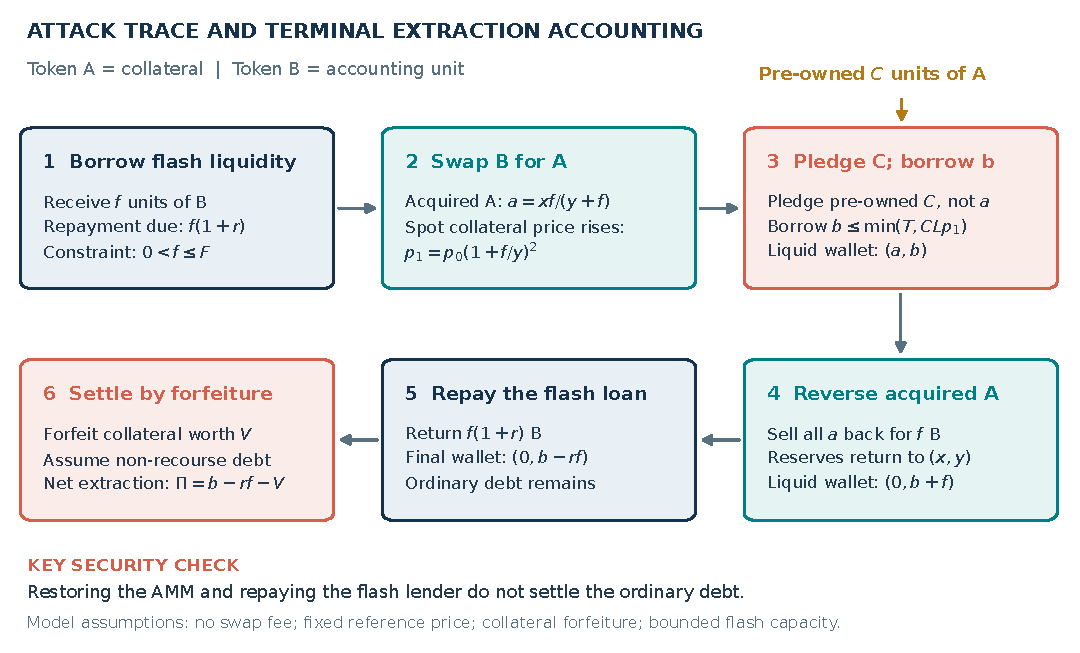
\includegraphics[width=0.97\textwidth]{figures/color-attack-flow.pdf}
\caption{Illustrated core attack schedule. The pre-owned collateral is separate
from the AMM tokens acquired during manipulation. Collateral forfeiture is the
settlement assumption that turns the residual lending debt into extraction.}
\label{fig:attack-visual}\end{figure}

\begin{table}[!ht]\centering
\caption{Constructed optimal example: attacker wallet and protocol state.}
\begin{tabular}{lrrrrl}\toprule
\textcolor{Navy}{Stage} & \textcolor{Navy}{Wallet $A$} & \textcolor{Navy}{Wallet $B$} & \textcolor{Navy}{AMM $x$} & \textcolor{Navy}{AMM $y$} & \textcolor{Navy}{Other obligation/state}\\\midrule
Initial & 100 & 0 & 1000 & 1000 & No debt\\
Flash acquisition & 100 & 1000 & 1000 & 1000 & Flash due: 1000.9 $B$\\
Manipulating swap & 600 & 0 & 500 & 2000 & Spot price: 4 $B/A$\\
Pledge and borrow & 500 & 300 & 500 & 2000 & Custody: 100 $A$; debt: 300 $B$\\
Reverse swap & 0 & 1300 & 1000 & 1000 & Ordinary debt persists\\
Repay flash loan & 0 & 299.1 & 1000 & 1000 & Flash obligation discharged\\
Forfeit collateral & 0 & 299.1 & 1000 & 1000 & Net extraction: 199.1 $B$\\
\bottomrule\end{tabular}\label{tab:ledger}\end{table}

The ledger uses $f=1000$, $C=100$, $L=0.75$, $r=0.0009$ and $T=400$.
The final wallet is 299.1 units of $B$, but initial wealth was worth 100 units.
Consequently, net extraction is 199.1 rather than 299.1. The lending protocol
holds collateral with reference value 100 against debt 300. Under the stipulated
settlement, the lender's 200-unit shortfall is split between attacker extraction
of 199.1 and the flash lender's fee of 0.9. No token conservation law is violated.

\takeaway{\textbf{Security interpretation.} Restoring AMM balances and repaying the
flash lender do not restore the attached lender's collateral coverage. Economic
safety must be checked across the whole modeled transaction.}

\clearpage
\subsection{\textcolor{Teal}{How a model becomes a verification result}}
The solver searches for any feasible execution with positive extraction. The
analytical calculation provides a separate criterion for the fixed core model,
while exact replay checks that a returned rational witness obeys its transitions.

\begin{figure}[!ht]\centering
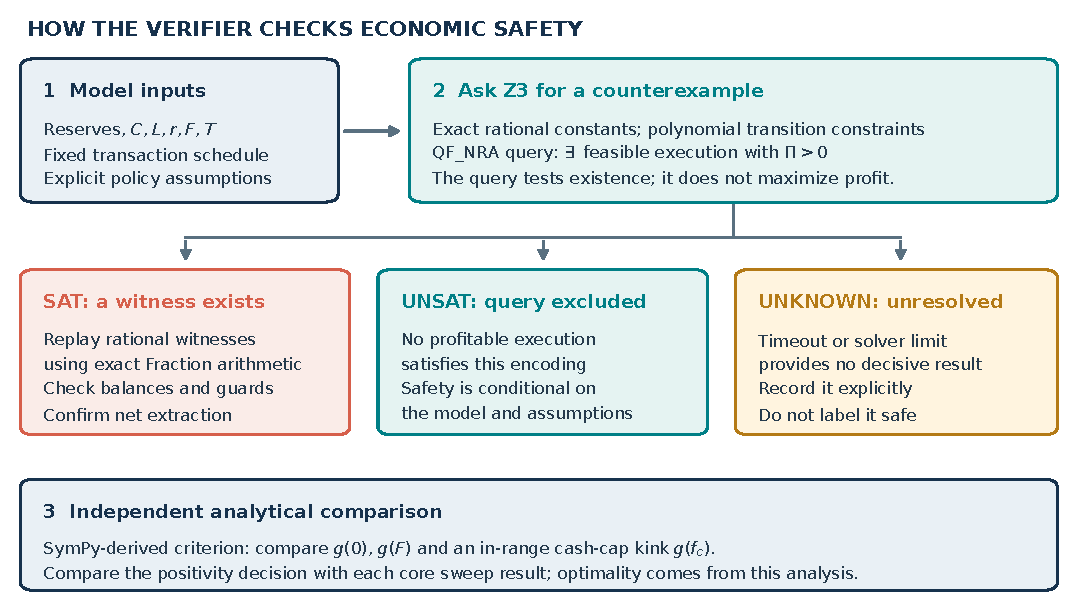
\includegraphics[width=0.97\textwidth]{figures/color-verification-pipeline.pdf}
\caption{Verification workflow. SAT, UNSAT and UNKNOWN carry different meanings.
The analytical criterion is specific to the capped core profit function. Exact
replay checks a witness; it is not an independently checked UNSAT certificate.}
\end{figure}

\begin{table}[!ht]\centering
\caption{Defenses, sufficient conditions, and limits of the evidence.}
\begin{tabular}{p{0.20\textwidth}p{0.35\textwidth}p{0.35\textwidth}}\toprule
\textcolor{Navy}{Defense} & \textcolor{Navy}{Required model condition} & \textcolor{Navy}{What remains to justify in practice}\\\midrule
Bounded oracle & $p_{\rm oracle}\leq p_0(1+\epsilon)$ and $L(1+\epsilon)\leq1$ & Show the concrete oracle enforces the assumed bound.\\
Rational dynamic LTV & $L(f)=L_0/(1+f/y)^2$, with $L_0<1$ & Establish how the relevant distortion is measured and enforced.\\
Sufficient reserve depth & $y\geq y_{\rm safe}$ for fixed $V,L,r,F,p_0$ & Justify collateral value, capacity and price assumptions.\\
Corrected vault minting & Use the proxy's true pre-deposit assets for share issuance & Verify the deployed vault's valuation and settlement rules.\\
Donation health guard & Post-donation collateral must cover debt at the given threshold & Model liquidation and all other routes to unhealthy debt.\\
\bottomrule\end{tabular}\end{table}

\takeaway{\textbf{Reading the labels.} SAT means the encoded target is reachable.
UNSAT excludes that target under the model's assumptions. UNKNOWN leaves the
question unresolved. A label is meaningful only together with the property checked.}

\clearpage
\subsection{\textcolor{Teal}{Measured decisions and solving-time distribution}}
Figure~\ref{fig:measured} separates the number of distinct parameter settings
from the number of solver calls. It also exposes the variation hidden by a
single median. Colors identify decisions; horizontal navy marks show medians.

\begin{figure}[!ht]\centering
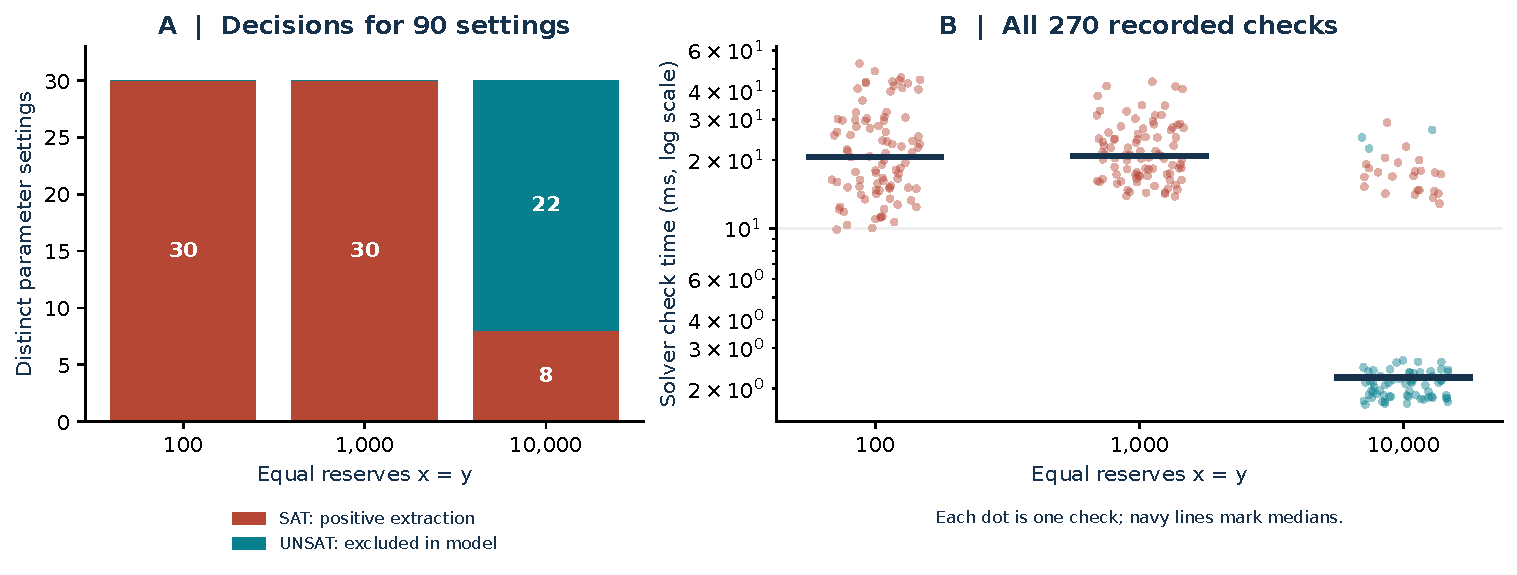
\includegraphics[width=0.98\textwidth]{figures/color-measured-overview.pdf}
\caption{Left: decisions for the 90 distinct settings. Right: solver-check time
for all 270 recorded calls on a logarithmic axis. There were no UNKNOWN results.
Each reserve group contains 30 settings and 90 calls.}
\label{fig:measured}\end{figure}

\begin{table}[!ht]\centering
\caption{Decision counts by distinct setting and descriptive timing statistics.}
\begin{tabular}{rrrrrrr}\toprule
\textcolor{Navy}{$x=y$} & \textcolor{Navy}{SAT settings} & \textcolor{Navy}{UNSAT settings} & \textcolor{Navy}{Min. ms} & \textcolor{Navy}{Median ms} & \textcolor{Navy}{P95 ms} & \textcolor{Navy}{Max. ms}\\\midrule
100 & 30 & 0 & 9.894 & 20.606 & 44.127 & 52.619\\
1,000 & 30 & 0 & 13.823 & 20.785 & 36.477 & 43.826\\
10,000 & 8 & 22 & 1.701 & 2.233 & 21.472 & 29.053\\
\bottomrule\end{tabular}\end{table}
The timing columns use all 90 calls at each reserve depth. P95 is the 95th
percentile with linear interpolation. It describes this sample; it is not a
confidence bound. Constraint construction and witness replay are outside these times.

\begin{table}[!ht]\centering
\caption{Experimental grid and counting rules.}
\begin{tabular}{lll}\toprule
\textcolor{Navy}{Dimension} & \textcolor{Navy}{Values} & \textcolor{Navy}{Count}\\\midrule
Equal reserve depth & 100; 1000; 10000 & 3\\
Loan-to-value limit & 0.50 to 0.95 in steps of 0.05 & 10\\
Flash fee rate & 0.09\%; 0.15\%; 0.30\% & 3\\
Fixed economic inputs & $C=100$, $F=1000$, $T=400$, $p_0=1$ & Constant\\
Distinct settings & $3\times10\times3$ & 90\\
Repeated solver calls & 3 per setting & 270\\
\bottomrule\end{tabular}\end{table}

\takeaway{\textbf{Observed pattern.} The deepest pool has 22 UNSAT settings out of
30; the other two depths have none in this grid. These proportions describe
selected synthetic settings, not the probability that a real protocol is attacked.}

\clearpage
\subsection{\textcolor{Teal}{Decision boundary and analytical profit curves}}
\begin{figure}[!ht]\centering
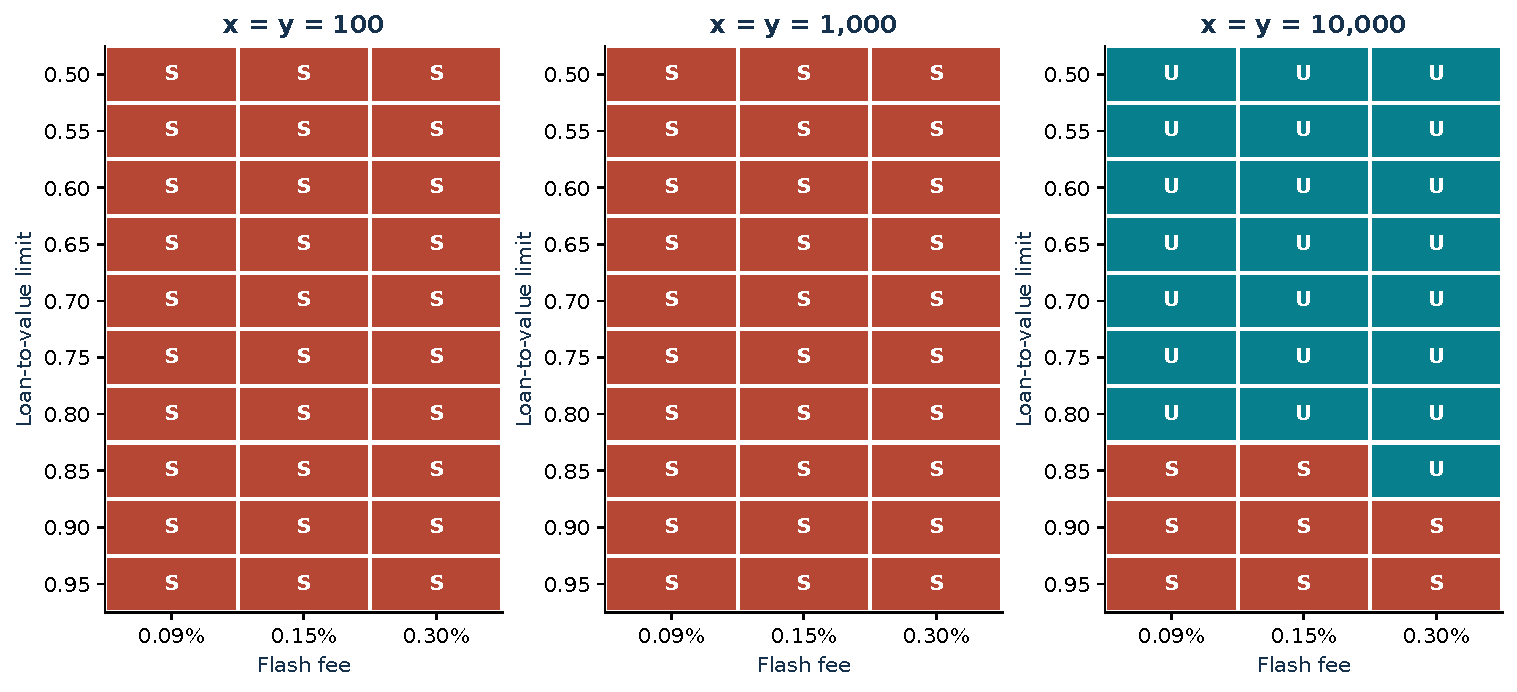
\includegraphics[width=0.98\textwidth]{figures/color-decision-map.pdf}
\caption{Recorded decision map. S (coral) denotes SAT and U (teal) denotes UNSAT.
Each cell is one parameter setting; all three repeats agree. Lower LTV and
greater reserve depth can exclude extraction within this fixed grid.}
\end{figure}

\begin{figure}[!ht]\centering
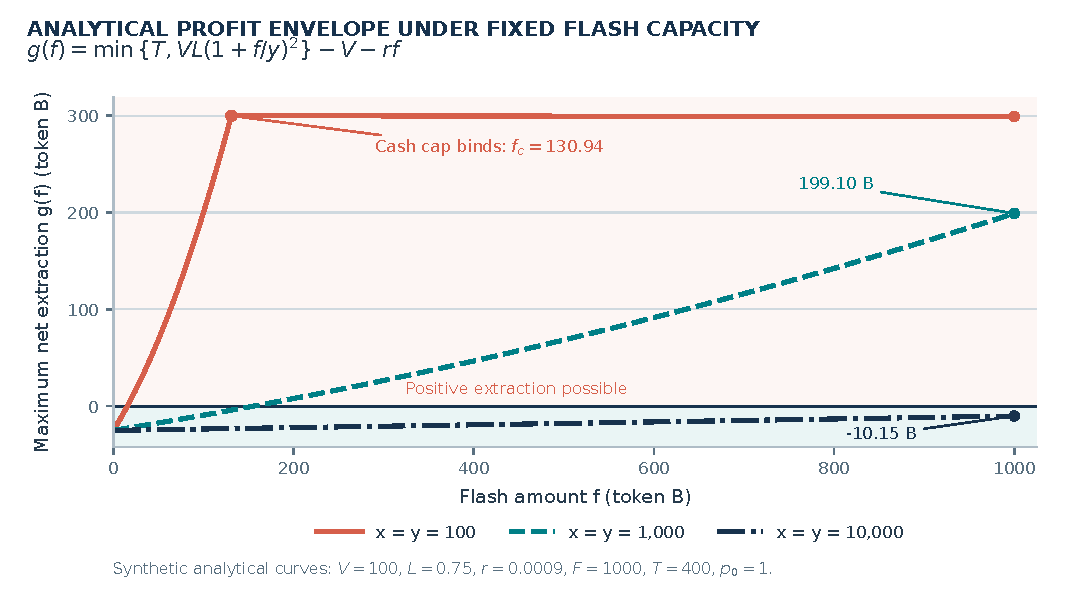
\includegraphics[width=0.92\textwidth]{figures/color-profit-curves.pdf}
\caption{Analytical illustration of $g(f)$, using $V=100$, $L=0.75$, $r=0.0009$,
$T=400$, $F=1000$ and the indicated reserve depth. This evaluates the derived
formula; the plotted points are not new solver measurements. The zero line
separates positive extraction from nonpositive net outcomes.}
\end{figure}

The shallow pool reaches the cash cap within the allowed interval. Beyond that
kink the marginal effect of another unit of flash liquidity is the negative
flash fee. At the baseline depth of 1000 the endpoint $f=1000$ yields 199.1.
At depth 10000 the entire curve stays below zero for the displayed LTV and fee.
The limit $f=0$ is included to visualize the analytical endpoint; a flash attack
in the core query requires $f>0$.

\clearpage
\appendices
\section{\textcolor{Navy}{Reproducibility and Output Evidence}}
The repository contains the model, test suite, raw CSV/JSON results, exported
SMT-LIB queries, and plotting scripts. From the project root, activate the
Python environment and execute the following commands in order:
\begin{verbatim}
python -m pip install -r requirements.txt
python -m pytest
python -m src.utils.benchmark --out results
python -m src.utils.plot_results --results results --paper paper
python -m src.utils.report --results results --paper paper
\end{verbatim}
Long commands may wrap visually; each command is one terminal input.
Compile this paper from the paper directory using two runs of
\texttt{pdflatex research-paper.tex}. References are embedded in the source,
so this edition does not require a BibTeX step.

Figures below are browser screenshots of an output viewer populated from
the saved project files. They preserve recorded outputs; they are not captures
of the user's VS Code session.\footnote{The test screenshot is sourced from
the saved test log. Its elapsed time belongs to that recorded run, not to a
new test execution performed for paper preparation.} Tables in the body provide
the corresponding searchable evidence. Timing changes between reruns are expected.

\begin{figure*}[!ht]\centering
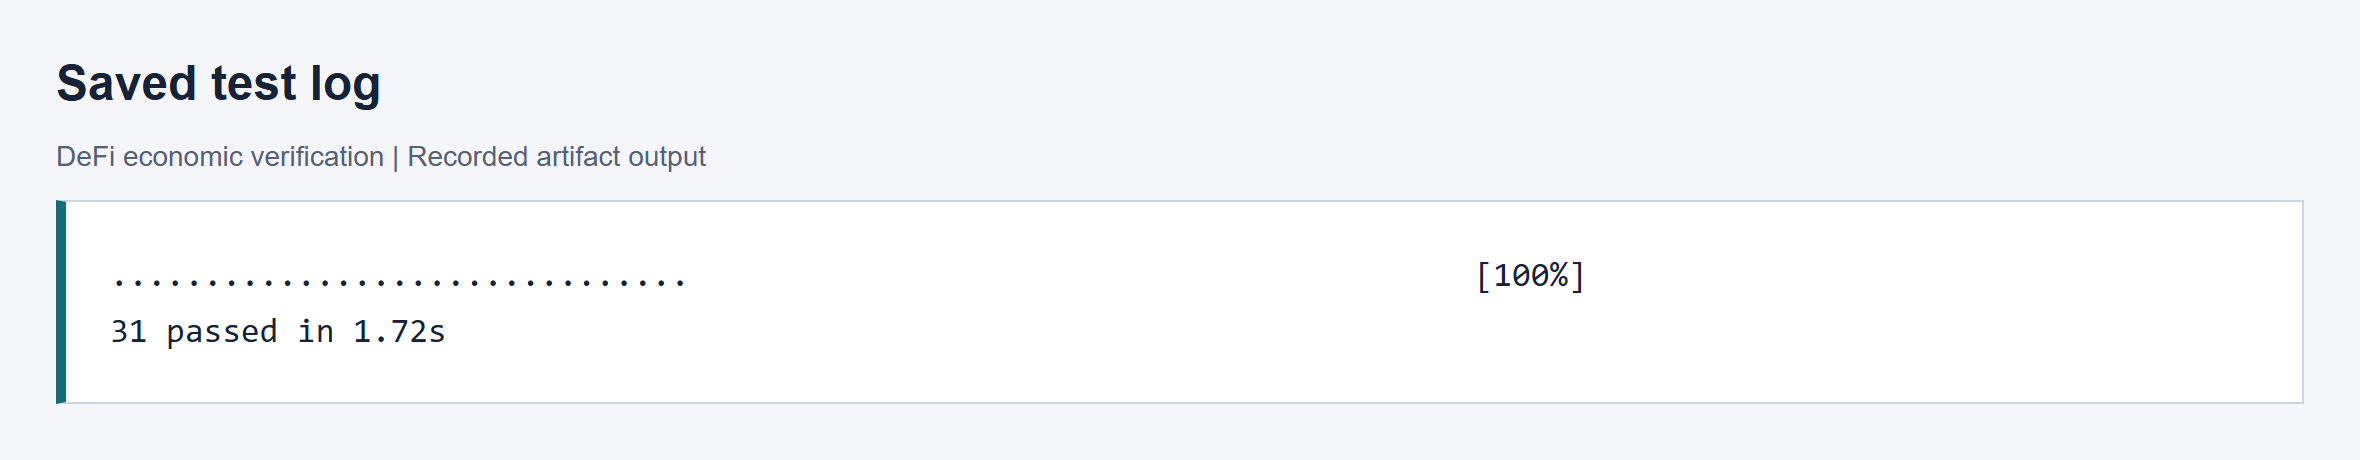
\includegraphics[width=0.92\textwidth]{figures/output-tests.png}
\caption{Saved automated-test output from results/test-run.txt: 31 tests passed.}
\end{figure*}
\begin{figure*}[!ht]\centering
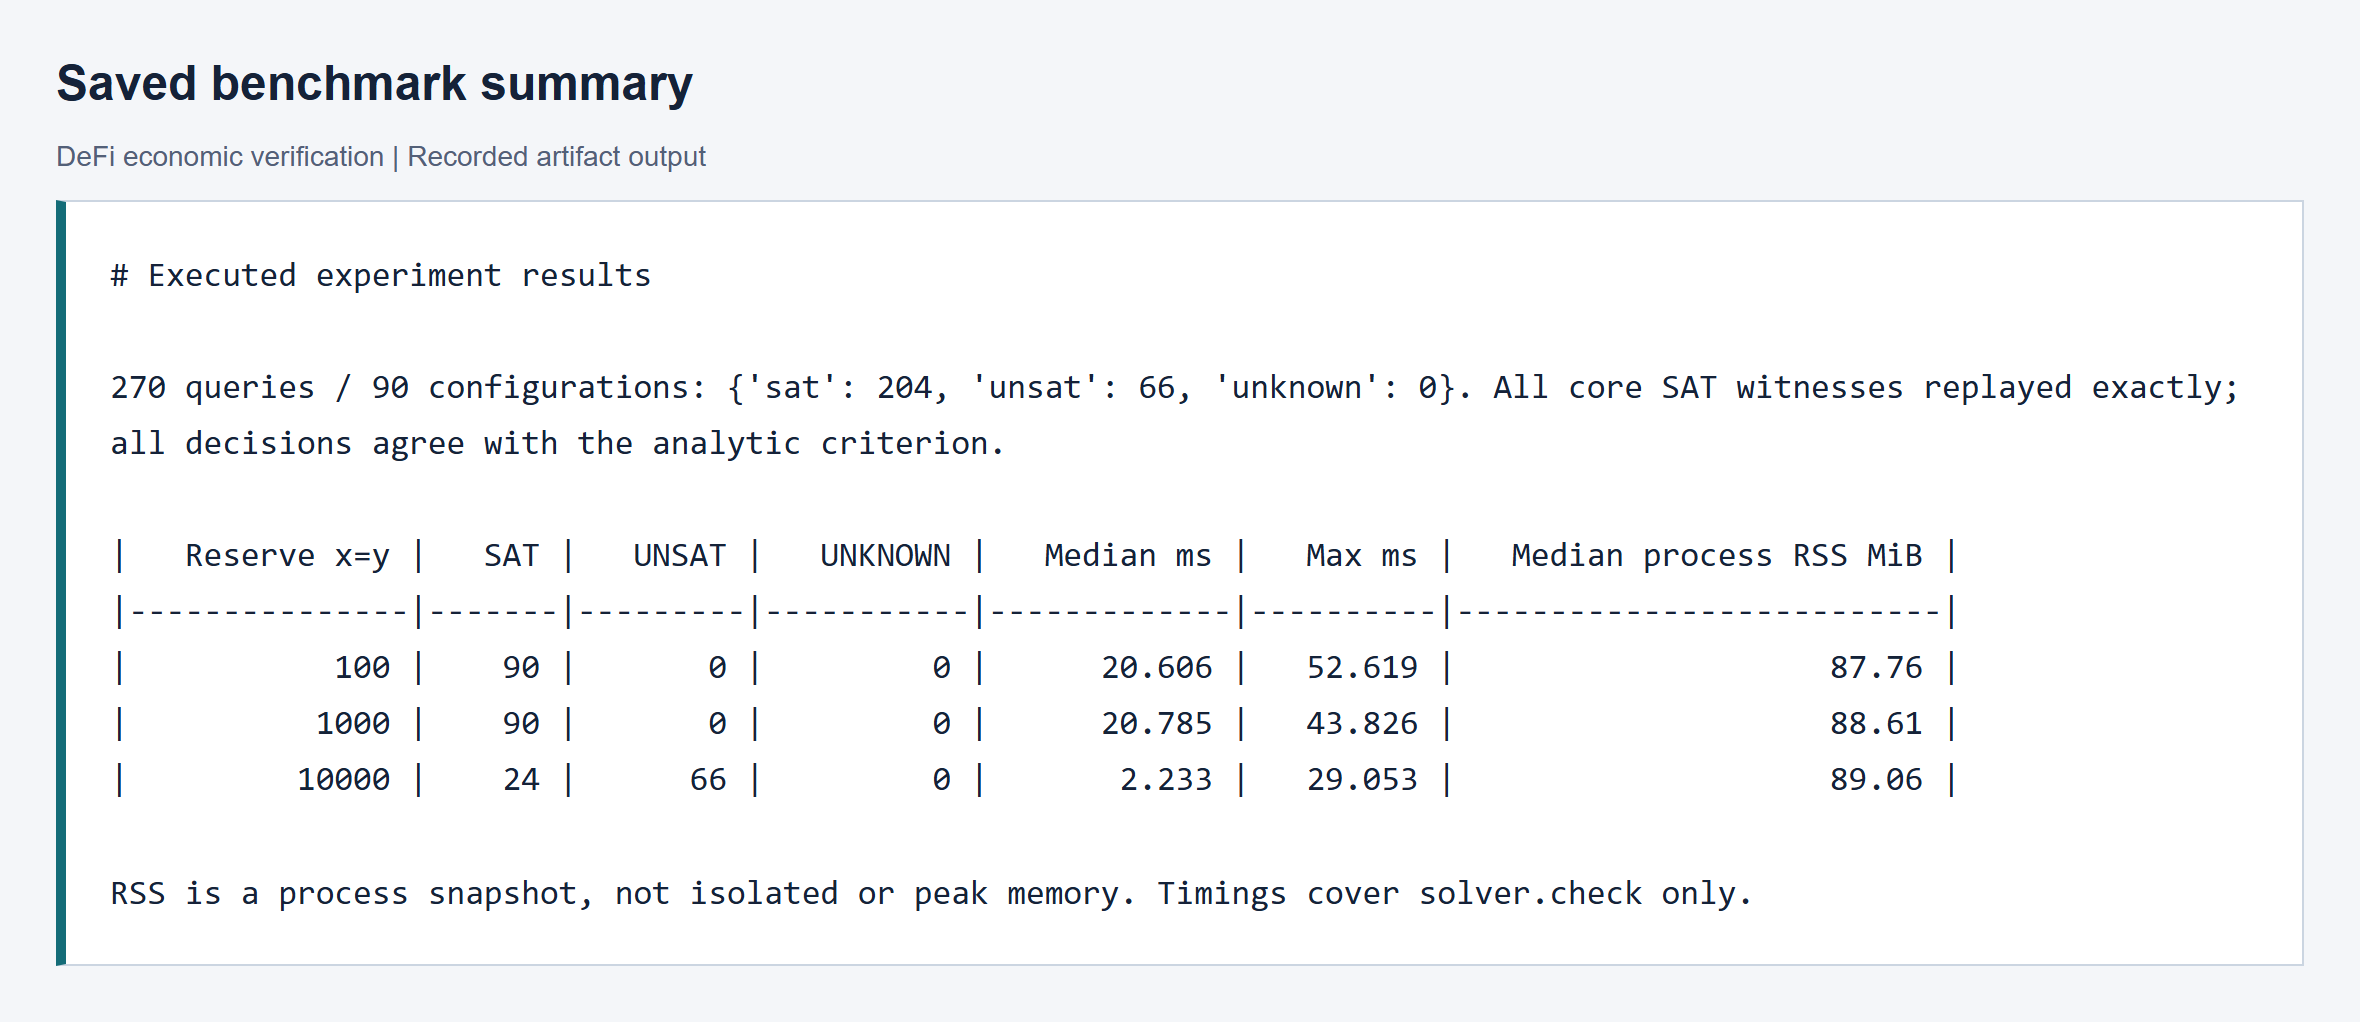
\includegraphics[width=0.92\textwidth]{figures/output-summary.png}
\caption{Recorded benchmark summary from results/SUMMARY.md, including counts,
solving times, and process memory snapshots.}
\end{figure*}
\begin{figure*}[!ht]\centering
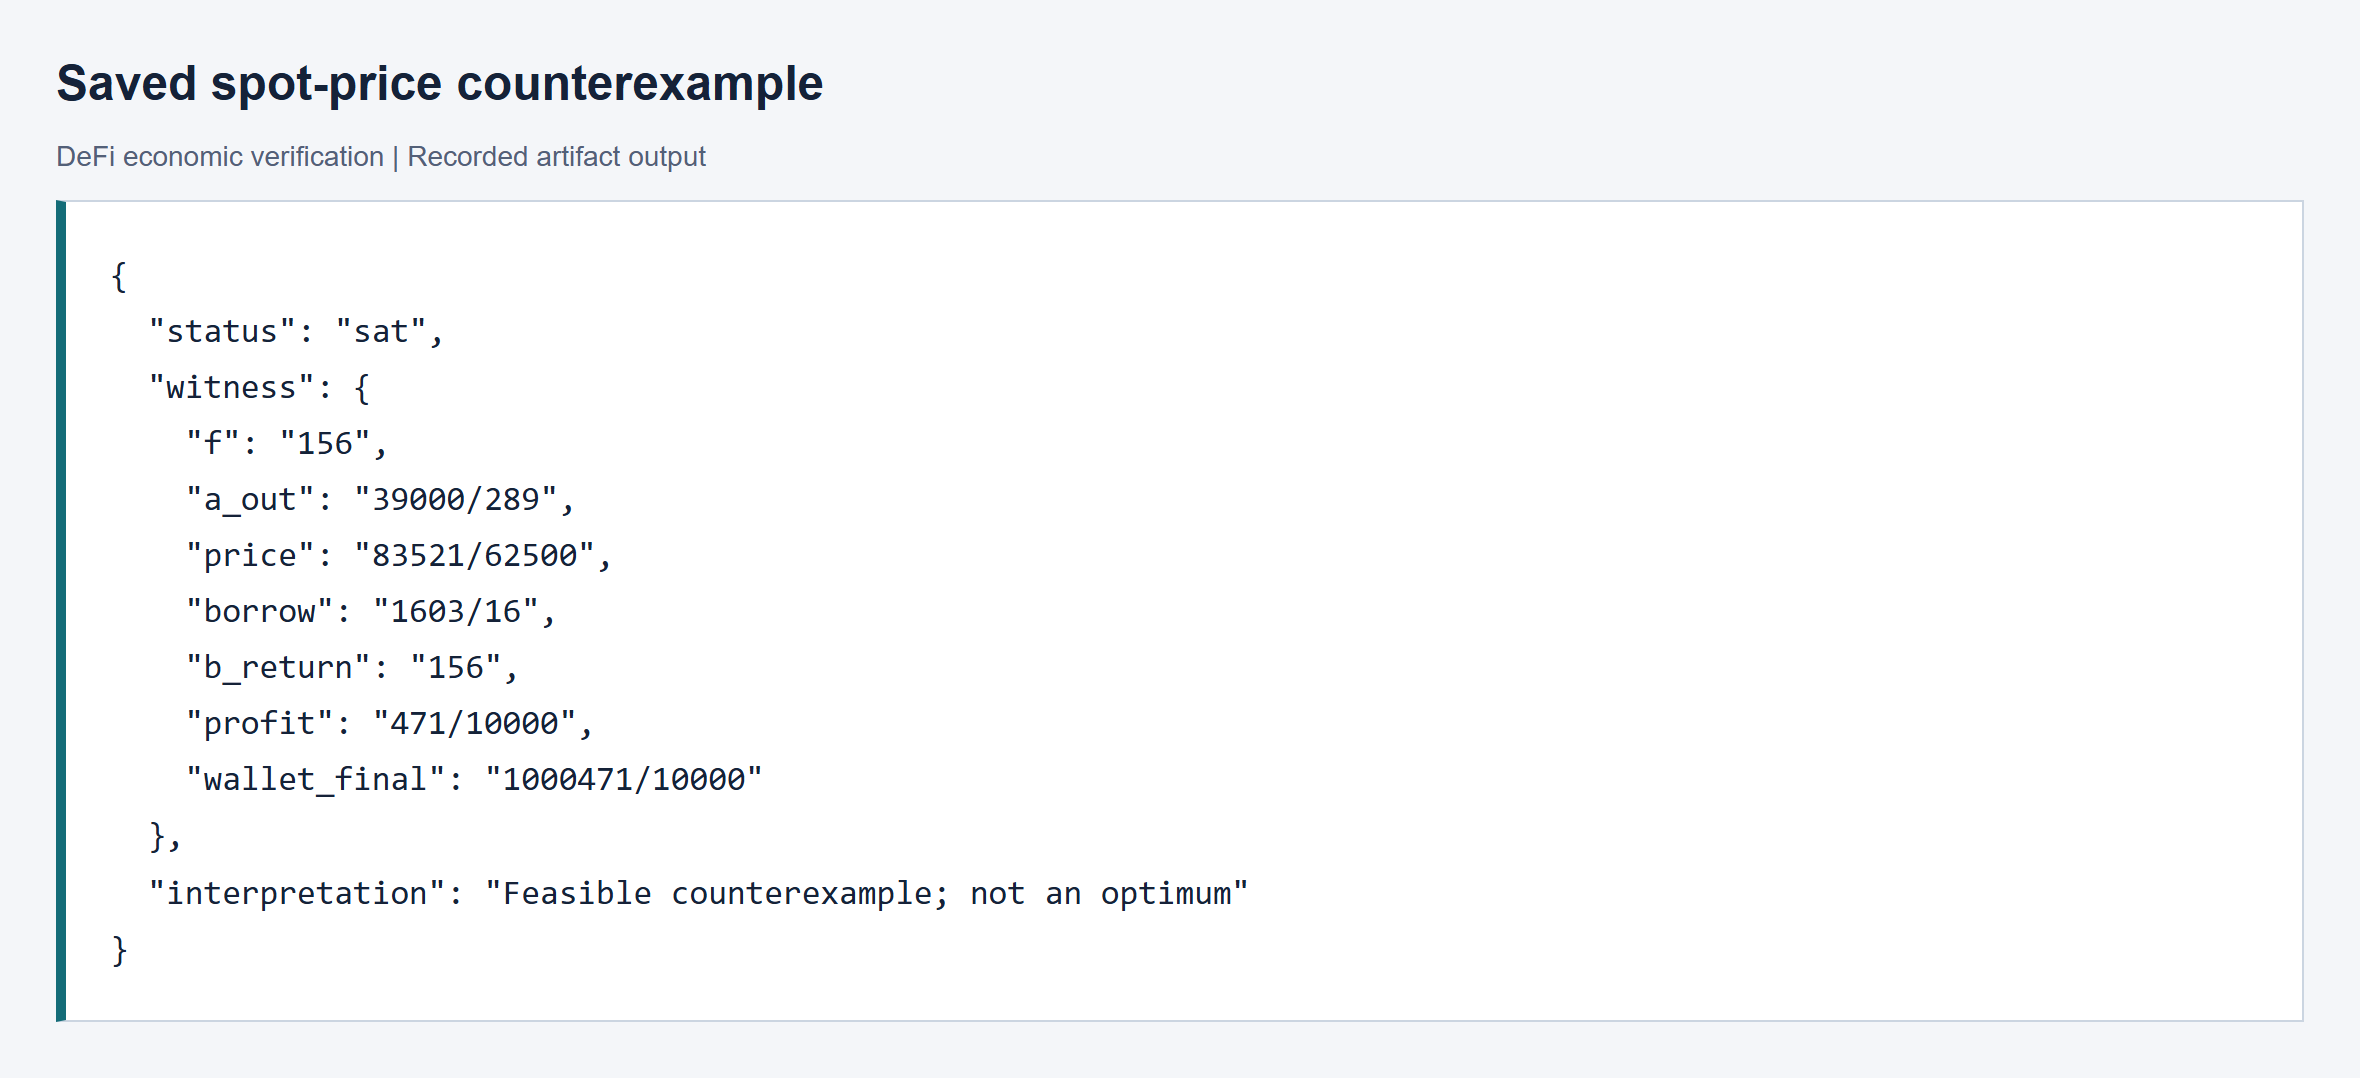
\includegraphics[width=0.92\textwidth]{figures/output-witness.png}
\caption{Exact spot-model witness fields from results/cases.json. Positive
profit establishes satisfiability; it does not establish optimality.}
\end{figure*}
\section{\textcolor{Navy}{Research Integrity and Artifact Scope}}
The prose and exposition were prepared for this project with AI assistance,
including assistance with code and manuscript drafting. The student ran the
project locally and compiled its LaTeX output. This statement does not claim
independent student authorship of every implementation detail. Any submission
should identify the student's own reviewed contributions and follow the
institution's disclosure requirements.

Historical mechanisms and prior systems are attributed in the references.
The measurements come from the local artifact, and synthetic quantities are
identified as such. No similarity score, plagiarism certification, or AI-detector
outcome is asserted. The main reproducibility boundary is semantic: agreement
between a solver and an analytical model cannot establish that an unmodeled
contract behaves identically.

\begin{thebibliography}{12}
\bibitem{qin} K. Qin et al., ``Attacking the DeFi Ecosystem with Flash Loans for Fun and Profit,'' 2020. \url{https://arxiv.org/abs/2003.03810}.
\bibitem{harvest} Harvest Finance, ``fUSDC/fUSDT Economic Attack Oct 26 2020.'' \url{https://docs.harvest.finance/other/security/incidents/fusdc-fusdt-economic-attack-oct-26-2020}.
\bibitem{euler} Euler Finance, ``War \& Peace: Behind the Scenes of Euler's \$240M Exploit Recovery.'' \url{https://www.euler.finance/blog/war-peace-behind-the-scenes-of-eulers-240m-exploit-recovery}.
\bibitem{z3} Microsoft, ``Online Z3 Guide: Python Introduction.'' \url{https://microsoft.github.io/z3guide/programming/Z3%20Python/Introduction/}.
\bibitem{uniswap} H. Adams et al., ``Uniswap v3 Core,'' 2021. \url{https://blog.uniswap.org/whitepaper-v3.pdf}.
\bibitem{defiposer} ``On the Just-In-Time Discovery of Profit-Generating Transactions in DeFi Protocols,'' 2021. \url{https://arxiv.org/abs/2103.02228}.
\bibitem{clockwork} ``Clockwork Finance: Automated Analysis of Economic Security in Smart Contracts,'' 2021. \url{https://arxiv.org/abs/2109.04347}.
\bibitem{foray} ``FORAY: Towards Effective Attack Synthesis against Deep Logical Vulnerabilities in DeFi Protocols,'' 2024. \url{https://arxiv.org/abs/2407.06348}.
\bibitem{oracle} ``Towards Verified Price Oracles for Decentralized Exchange Protocols,'' FMBC, 2021. \url{https://drops.dagstuhl.de/entities/document/10.4230/OASIcs.FMBC.2021.1}.
\bibitem{slither} Crytic, ``Slither.'' \url{https://github.com/crytic/slither}.
\bibitem{mythril} Consensys Diligence, ``MythX Tech: Behind the Scenes of Smart Contract Security Analysis,'' 2019. \url{https://diligence.consensys.io/blog/2019/12/mythx-tech-behind-the-scenes-of-smart-contract-security-analysis/}.
\end{thebibliography}
\end{document}


